\documentclass[10pt, landscape]{article}
\usepackage[scaled=0.92]{helvet}
\usepackage{calc}
\usepackage{multicol}
\usepackage[a4paper,margin=3mm,landscape]{geometry}
\usepackage{amsmath,amsthm,amsfonts,amssymb}
\usepackage{color,graphicx,overpic}
\usepackage{hyperref}
\usepackage{newtxtext} 
\usepackage{enumitem}
\usepackage[table]{xcolor}
\usepackage{mathtools}
\setlist{nosep}
% for including images
\graphicspath{ {./images/} }

\pdfinfo{
  /Title (is2218_finals_cheatsheet.pdf)
  /Creator (TeX)
  /Producer (pdfTeX 1.40.0)
  /Author (Gavin Chiam)
  /Subject (IS2218)
/Keywords (is2218, nus, cheatsheet, pdf)}

% Turn off header and footer
\pagestyle{empty}

% redefine section commands to use less space
\makeatletter
\renewcommand{\section}{\@startsection{section}{1}{0mm}%
  {-1ex plus -.5ex minus -.2ex}%
  {0.5ex plus .2ex}%x
{\normalfont\large\bfseries}}
\renewcommand{\subsection}{\@startsection{subsection}{2}{0mm}%
  {-1explus -.5ex minus -.2ex}%
  {0.5ex plus .2ex}%
{\normalfont\normalsize\bfseries}}
\renewcommand{\subsubsection}{\@startsection{subsubsection}{3}{0mm}%
  {-1ex plus -.5ex minus -.2ex}%
  {1ex plus .2ex}%
{\normalfont\small\bfseries}}%
\makeatother

\renewcommand{\familydefault}{\sfdefault}
\renewcommand\rmdefault{\sfdefault}
%  makes nested numbering (e.g. 1.1.1, 1.1.2, etc)
\renewcommand{\labelenumii}{\theenumii}
\renewcommand{\theenumii}{\theenumi.\arabic{enumii}.}
\renewcommand\labelitemii{•}
\renewcommand\labelitemiii{•}

\definecolor{mathblue}{cmyk}{1,.72,0,.38}
\everymath\expandafter{\the\everymath \color{mathblue}}

% Don't print section numbers
\setcounter{secnumdepth}{0}

\setlength{\parindent}{0pt}
\setlength{\parskip}{0pt plus 0.5ex}
%% adjust spacing for all itemize/enumerate
\setlength{\leftmargini}{0.4cm}
\setlength{\leftmarginii}{0.4cm}
\setlength{\leftmarginiii}{0.2cm}
\setlist[itemize,1]{leftmargin=2mm,labelindent=1mm,labelsep=1mm}
\setlist[itemize,2]{leftmargin=4mm,labelindent=1mm,labelsep=1mm}
\setlist[itemize,3]{leftmargin=4mm,labelindent=1mm,labelsep=1mm}

% adding my commands
\input{../../commands/style-helpers.tex}
\makeatletter
\newcommand*{\xdashrightarrow}[2][]{%
  \mathrel{%
    \mathpalette{\da@xarrow{#1}{#2}{}\da@rightarrow{\,}{}}{}%
  }%
}
\newcommand*{\da@rightarrow}{\mathchar"0\hexnumber@\symAMSa 4B }
\newcommand*{\da@xarrow}[7]{%
  % #1: below
  % #2: above
  % #3: arrow left
  % #4: arrow right
  % #5: space left 
  % #6: space right
  % #7: math style 
  \sbox0{$\ifx#7\scriptstyle\scriptscriptstyle\else\scriptstyle\fi#5#1#6\m@th$}%
  \sbox2{$\ifx#7\scriptstyle\scriptscriptstyle\else\scriptstyle\fi#5#2#6\m@th$}%
  \sbox4{$#7\dabar@\m@th$}%
  \dimen@=\wd0 %
  \ifdim\wd2 >\dimen@
    \dimen@=\wd2 %   
  \fi
  \count@=2 %
  \def\da@bars{\dabar@\dabar@}%
  \@whiledim\count@\wd4<\dimen@\do{%
    \advance\count@\@ne
    \expandafter\def\expandafter\da@bars\expandafter{%
      \da@bars
      \dabar@ 
    }%
  }%  
  \mathrel{#3}%
  \mathrel{%   
    \mathop{\da@bars}\limits
    \ifx\\#1\\%
    \else
      _{\copy0}%
    \fi
    \ifx\\#2\\%
    \else
      ^{\copy2}%
    \fi
  }%   
  \mathrel{#4}%
}
\makeatother

% -----------------------------------------------------------------------

\begin{document}
\raggedright
\footnotesize
\begin{multicols*}{4}
  % multicol parameters
  \setlength{\columnseprule}{0.25pt}

  \begin{center}
    \fbox{%
      \parbox{0.8\linewidth}{\centering \textcolor{black}{
          {\Large\textbf{IS2218 (Finals)}}
        \\ \normalsize{AY25/26 SEM 1}}
        \\ {\footnotesize \textcolor{gray}{github/Gavino3o}}
      }%
    }
  \end{center}

  \section{Time Value of Money}

  \begin{itemize}
    \item \textbf{Future Value (FV)}: Amount an investment will grow after earning interest
    \item \textbf{Present Value (PV)}: Current value of a future amount
    \item \textbf{Discount Factor (DF)}: Present value of a \$1 future payment
    \item \textbf{Discount Rate}: Interest rate used to compute present values of future cash flows
    \item \textbf{Discounted Cash Flow (DCF)}: Valuation method of calculating present value by discounting future cash flows
  \end{itemize}

  \subsection{Perpetuities and Annuities}

  \begin{itemize}
    \item \textbf{Perpetuity}: A stream of equal payments that continues forever
    \item \textbf{Annuity}: A stream of equal payments at regular intervals for a fixed period of time
    \item \textbf{Perpetuity Value}: Present value of a perpetuity, where $C$ is the cash payment per period and $r$ is the discount rate
    \item \textbf{Annuity Value}: Present value of an annuity, where $C$ is the cash payment per period, $r$ is the discount rate, and $t$ is the number of periods
    \item \textbf{PV Annuity Factor (PVAF)}: The present value of \$1 a year for each of $t$ years
    \item \textbf{FV Annuity Payment (FVAP)}: Future value of a series of equal payments made at the end of each period, where $C$ is the cash payment per period, $r$ is the discount rate, and $t$ is the number of periods
    \item \textbf{Annuity Due}: An annuity where payments are made at the beginning of each period instead of the end. Tip: Multiply the ordinary annuity value by $(1 + r)$ to get the annuity due value
    \item \textbf{Amortization}: The process of spreading out a loan into a series of fixed payments over time
    \item \textbf{Amortization Schedule}: A table that details each periodic payment on an amortizing loan, showing the amount applied to principal and interest, as well as the remaining balance after each payment \newline
    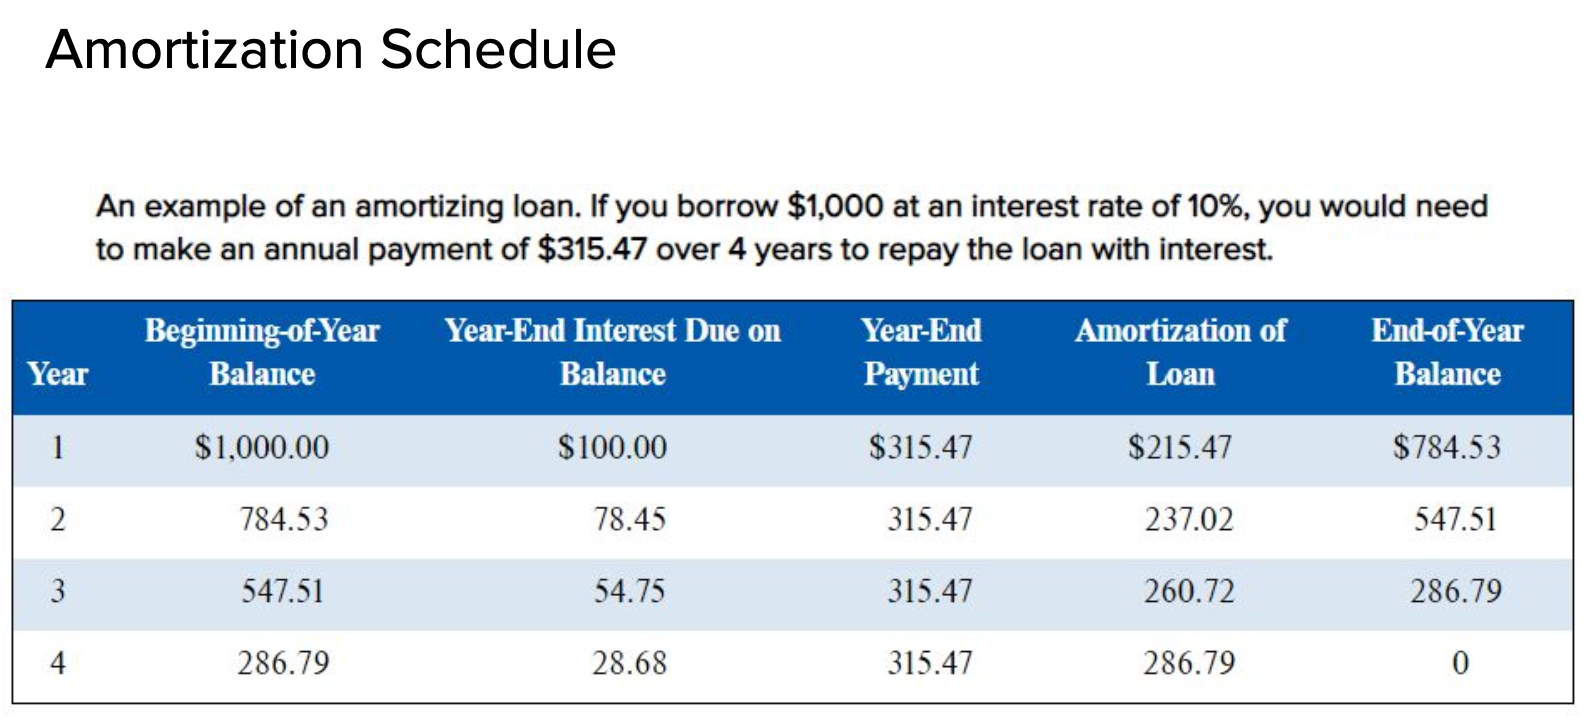
\includegraphics[width=0.97\linewidth]{../images/amortization_schedule.png} 
    \item \textbf{Effective Annual Rate (EAR)}: The actual annual rate that an investor earns (or pays) after accounting for compounding over a given period
    \item \textbf{Annual Percentage Rate (APR)}: The annual rate charged for borrowing or earned through an investment, without taking compounding into account (simple interest)
    \item \textbf{Monthly Rate (MR)}: The interest rate for a loan or investment calculated on a monthly basis
  \end{itemize}

  \subsection{Inflation}

    \begin{itemize}
      \item \textbf{Inflation}: The rate at which the general level of prices for goods and services is rising, leading to a decrease in purchasing power
      \item Current dollar cash flows must be discounted by the nominal interate rate
      \item \textbf{Nominal interest rate}: The stated interest rate on a loan or investment, not adjusted for inflation
      \item Real cash flows must be discounted by the real interest rate
      \item \textbf{Real interest rate}: The interest rate that has been adjusted to remove the effects of inflation, reflecting the true cost of borrowing or the true yield on an investment
      \item We can use inflation rate to calculate the future value of money. Just use it as the interest rate in the FV formula
    \end{itemize}

  \subsection{Formulas}
    \begin{itemize}
      \item \( \textbf{Future Value, } FV = PV (1 + r)^t \)
      \item \( \textbf{Present Value, } PV = \frac{\text{Future Value after t periods}}{(1 + r)^t} \)
      \item \( \textbf{Discount Factor, } DF = \frac{1}{(1 + r)^t} \)
      \item \( \textbf{Perpetuity Value, } PV = \frac{C}{r} \)
      \item \( \textbf{Annuity Value, } PV = C \times \left[ \frac{1 - (1 + r)^{-t}}{r} \right] \)
      \item \( \textbf{Annuity Value, } PV = C \times \left[ \frac{1}{r} - \frac{1}{r(1+r)^t} \right] \)
      \item \( \textbf{PV Annuity Factor (PVAF)} = \left[ \frac{1}{r} - \frac{1}{r(1+r)^t} \right]\)
      \item \( \textbf{FV Annuity Payment (FVAP)} = \left[ C \times PVAF \right] \times (1+r)^t\)
      \item \( \textbf{FV Annuity Payment (FVAP)} = C \times \left[ \frac{(1+r)^t - 1}{r} \right]\)
      \item \( PV_{\text{Annuity Due}} = PV_{\text{Annuity}} \times (1 + r) \)
      \item \( FV_{\text{Annuity Due}} = FV_{\text{Annuity}} \times (1 + r) \)
      \item \( \textbf{Loan Payment, } C = \frac{PV \times r}{1 - (1 + r)^{-t}} \)
      \item \( EAR = (1 + MR)^{12} - 1\)
      \item \( APR = MR \times 12 \)
      \item \( EAR = \left[ 1 + \frac{APR}{t} \right]^t - 1\)
      \item \( 1 + \text{real interest rate} = \frac{1 + \text{nominal interest rate}}{1 + \text{inflation rate}}\)
      \item \( \text{real interest rate} \approx \text{nominal interest rate} - \text{inflation rate} \)
      \item \( \text{Real Value} = \frac{\text{Nominal Value}}{(1 + \text{Inflation Rate})^t}\)
    \end{itemize}

  \section{Marketing}

  \begin{itemize}
    \item \textbf{Definition}: Activity, set of institutions, and processes for creating, communicating, delivering, and exchanging offerings that have value for customers, clients, partners, and society at large.
    \item Needs: States of felt deprivation (physical, social, individual)
    \item Wants: The form human needs take as they are shaped by society, culture and individual personality
    \item Demands: Human wants that are backed by buying power
    \item Marketing: Delivering Value to Customers, and in turn Capturing Value from Customers
    \item \textbf{Marketing Myopia}: Focusing on the product rather than the underlying customer needs
    \item \textbf{Production Concept:} Focus on production and distribution efficiency. Assumes consumers prefer products that are widely available and affordable. Appropriate when demand exceeds supply, or when production costs are high and improved productivity can lower prices. Impersonal, insensitive to customer needs.
    \item \textbf{Product Concept:} Focus on making continued product innovations. Assumes consumers favor products that offer the most quality, performance, or innovative features. Can lead to marketing myopia.
    \item \textbf{Selling Concept:} Focus on selling and promotion. Assumes consumers will not buy enough of the firm's products unless stimulated aggresively. Typically practiced with unsought goods (e.g. insurance, blood donations). Can lead to high risks, high costs, and unscrupulous image.
    \item \textbf{Marketing Concept:} Determine the needs and wants of target markets and delivering them more effectively and efficiently than competitors. 
      \begin{itemize}
        \item Crate, build, and maintain beneficial exchanges with target buyers to achieve organizational goals
        \item Fcous on buyer's needs vs the seller's needs
        \item Adapt and anticipate changes in consumer needs and characteristics
        \item Recognise needs not just product-based
        \item Stress regular consumer research and analysis
        \item Resource allocation to make goods and services desired by consumers
      \end{itemize}
    \item \textbf{Customer Driven} $\rightarrow$ Understand customers deeply about what they want $\rightarrow$ Create products that meet current needs
    \item \textbf{Customer Driving} $\rightarrow$ Understand customers even better than they understand themselves $\rightarrow$ Create products that meet needs now and in the future
    \item \textbf{Customer Relationship Management (CRM)}: Overall process of building and maintaining profitable customer relationships by delivering superior customer value and satisfaction. Not everyone is a desirable customer. Attract, keep, and grow profitable customers.\newline
    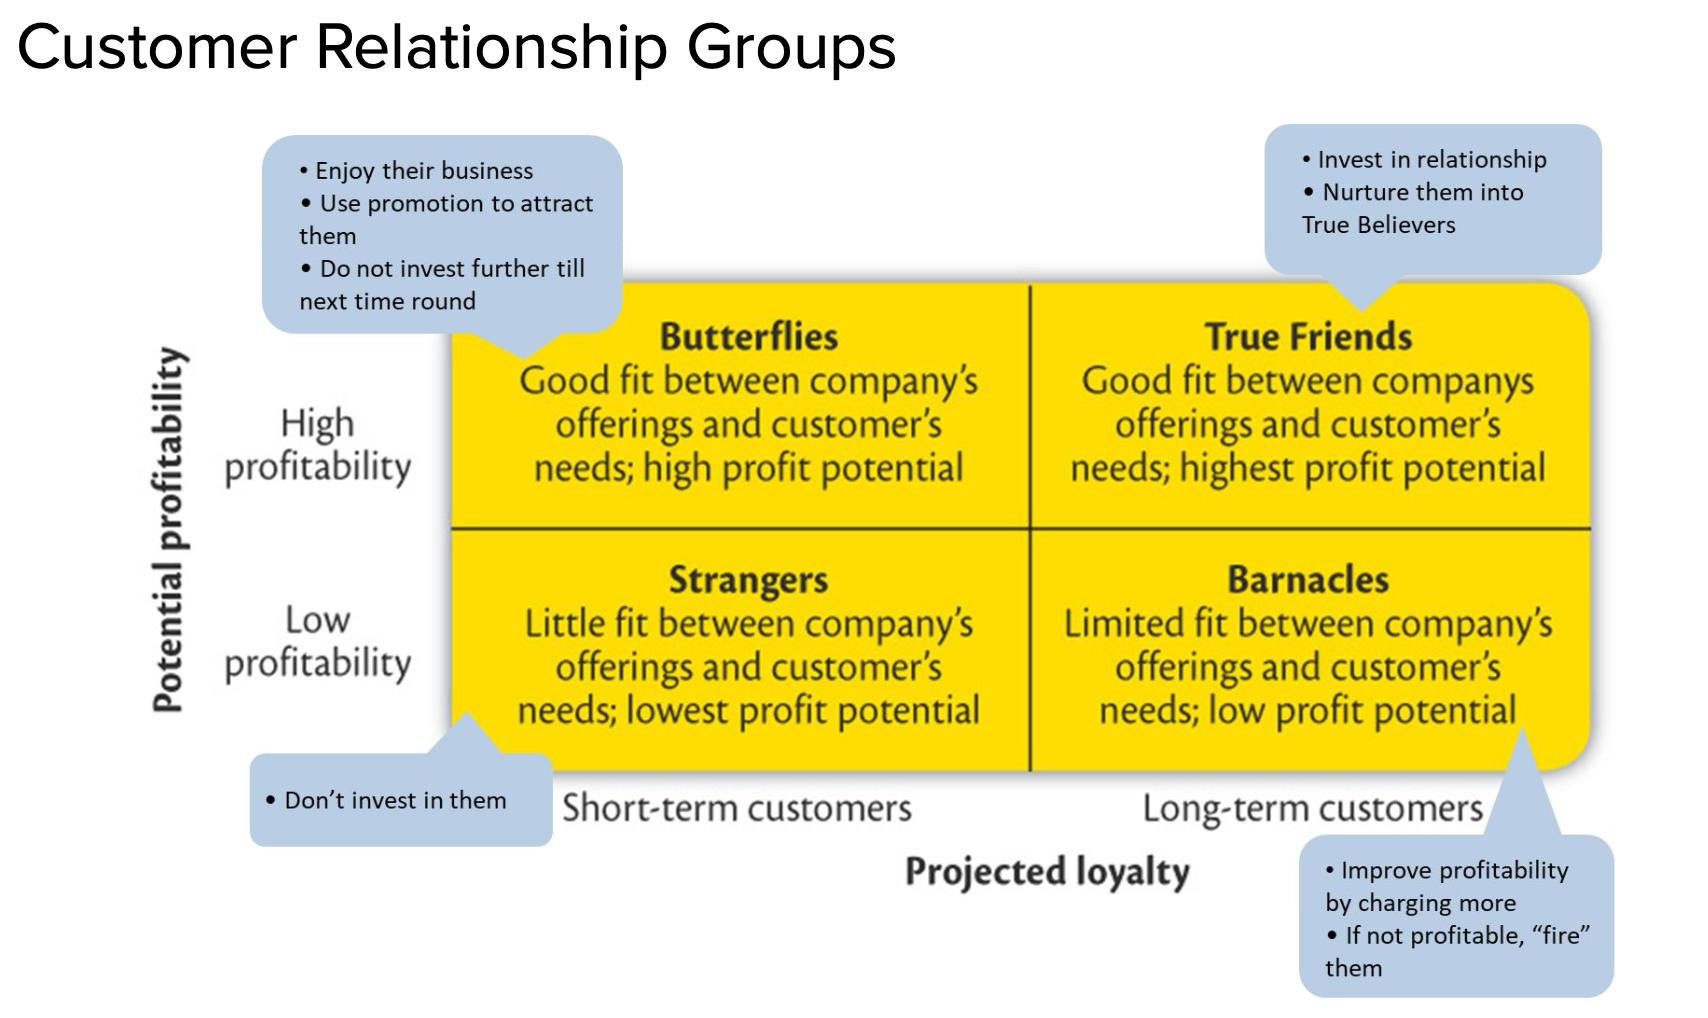
\includegraphics[width=0.97\linewidth]{../images/crg.png}
    
    \subsection{Marketing Process}
    \begin{enumerate}
      \item Understand the marketplace and customer needs and wants
        \begin{itemize}
          \item Research consumers and the marketplace (Qualitative and Quantitative)
          \item Manage marketing information and customer data
        \end{itemize}
      \item Design a customer-driven marketing strategy
      \begin{itemize}
        \item Market segementation and targeting
        \item Differentiation and positioning
      \end{itemize}
      \item Construct a marketing program that delivers superior value
      \begin{itemize}
        \item Product, Price, Place/Distribution, Promotion
      \end{itemize}
      \item Build profitable relationships and create customer delight
      \begin{itemize}
        \item Customer Relationship Management
        \item Marketing Partner Relationship Management
      \end{itemize}
      \item Capture value from customers to create profits and customer equity
      \begin{itemize}
        \item Create customer loyalty and retention
        \item Capture customer lifetime value
        \item Increase share of market and share of customer
      \end{itemize}
      \item In the midst: Harness marketing technology; Manage global markets; Ensure ethical and social responsibility
    \end{enumerate}

    % 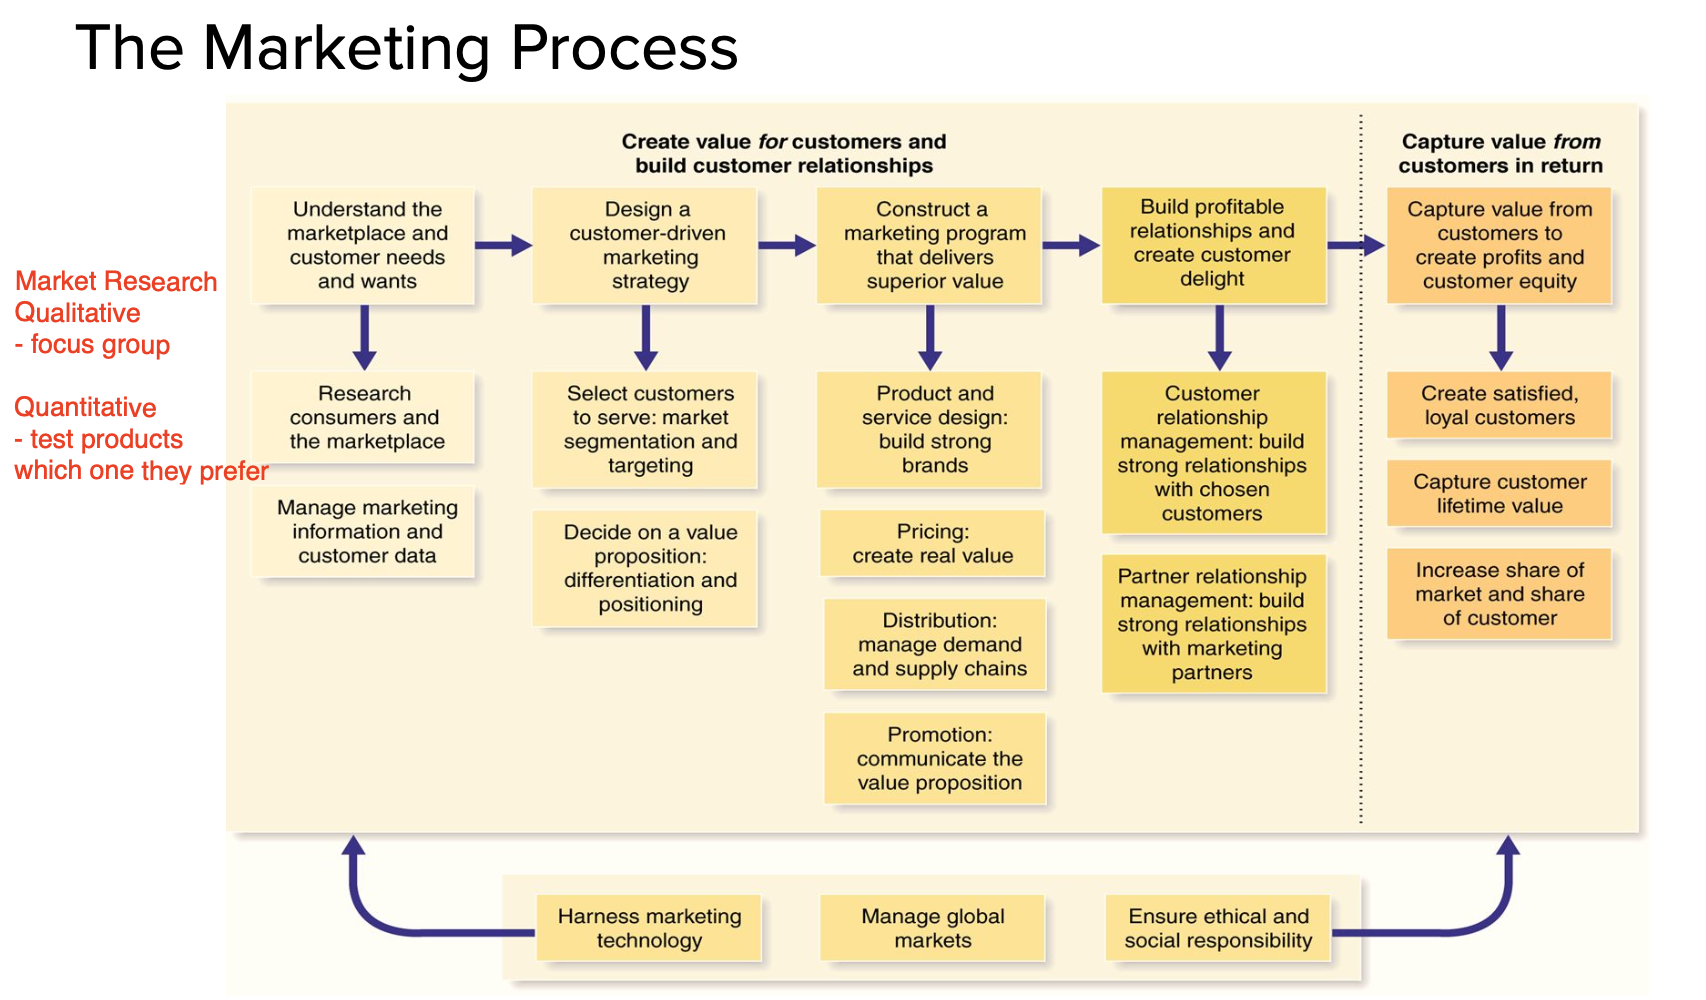
\includegraphics[height=0.8\linewidth, width=185px, angle=90]{../images/marketing_process.png}


  \end{itemize}

  \subsection{Marketing Management Process}
    \begin{enumerate}
      \item \textbf{Analyse and identify market oppurtunities}
      \begin{itemize}
        \item Marketing Research and Information Systems
        \item Marketing Environment Scanning
        \item Consumer and Business markets
      \end{itemize}
      \item \textbf{Research and select target markets}
      \begin{itemize}
        \item Measuring and forecasting demand
        \item Market segmentation, targeting, and positioning
      \end{itemize}
      \item \textbf{Develop marketing mix (4Ps): Product, Price, Place, Promotion}
      \item \textbf{Managing the marketing effort}
      \begin{itemize}
        \item Analysis (SWOT): Strengths, Weaknesses, Opportunities, Threats
        \item Planning (Setting objectives, marketing strategy)
        \item Implementation (Process of turning marketing strategy into action)
        \item Control (Evaluating results, taking corrective action)
      \end{itemize}
    \end{enumerate}
    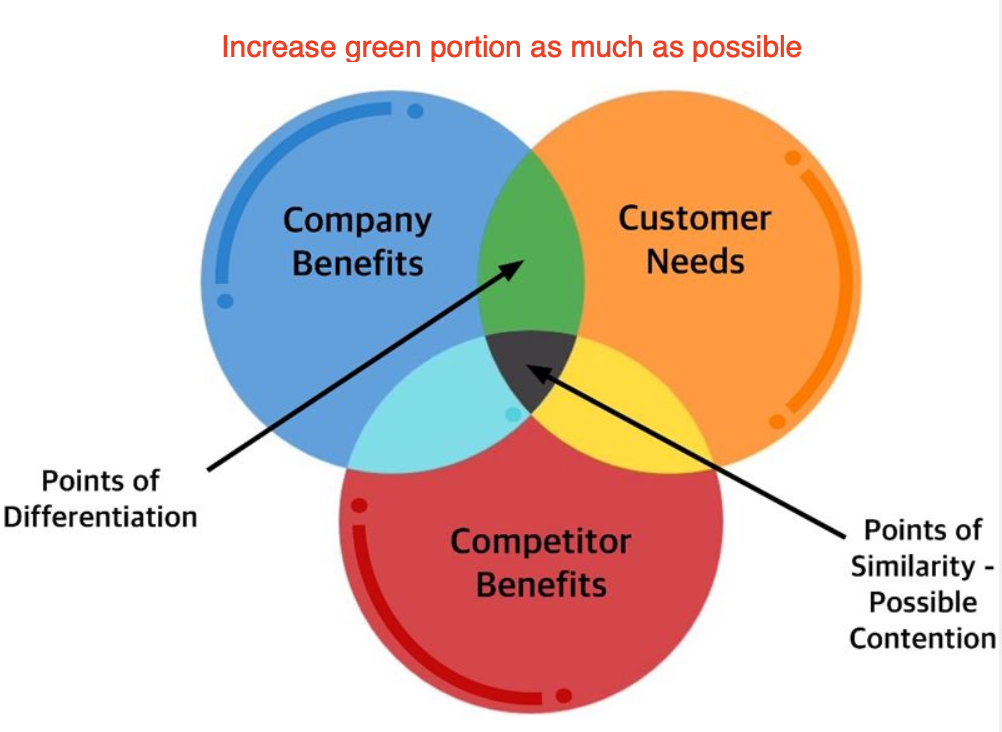
\includegraphics[width=0.80\linewidth, height = 100px]{../images/marketing_takeaway.png}

  \subsection{Bottom of the Pyramid (BOP)}
  \begin{itemize}
    \item \textbf{Definition}: The largest, but poorest socio-economic group in the world, consisting of approximately 4 billion people who live on less than \$2.50 per day.
    \item These markets are in the earliest stages of economic development, growth can be extremely rapid
    \item The competitive necessity of maintaining a low cost structure in these areas can push companies to discover creative ways to configure their products, finances, and supply chains to enhance productivity
    \item Hot-beds of commercial and technological experimentation
  \end{itemize}

  \subsection{Segmentation, Targeting, Positioning (STP)}
  \begin{itemize}
    \item \textbf{Segmentation}: Dividing a market into smaller groups with distinct needs, characteristics, or behaviors who might require separate products or marketing mixes. A market segment consists of consumers who respond in a similar way to a given set of marketing efforts.
    \item \textbf{Targeting}: Evaluating each market segment's attractiveness and selecting one or more segments to enter.
    \item \textbf{Positioning}: Arranging for a product to occupy a clear, distinctive, and desirable place relative to competing products in the minds of target consumers.
    \item \textbf{Differentiation}: Actually differentiating the market offering to create superior customer value.
    \item Don't have too many factors in positioning, or it will be confusing for customers
    \item Positioniong is perception based. Create a perception in the minds of customers about the product 
  \end{itemize}

  \section{Customer Lifetime Value (CLV)}

  \begin{enumerate}
    \item \textbf{Operational Excellence}: Providing customers with reliable products or services at competitive prices and delivered with minimal difficulty or inconvenience. Focus on efficiency of operations and processes. (e.g. Walmart, McDonald's)
    \item \textbf{Product Leadership}: Offering customers leading-edge products and services that consistently enhance the customer's use or application of the product, thereby making rivals' goods obsolete. Focus on innovation and product development. (e.g. Apple, Tesla)
    \item \textbf{Customer Intimacy}: Segmenting and targeting markets precisely, then tailoring offerings to match exactly the needs of those niches. Focus on customer service and building long-term relationships. (e.g. Amazon, Nordstrom)
  \end{enumerate}
  Aim to be best in one of the three value disciplines, and meet industry standards in the other two

  \subsubsection{Product Centric Business Model}
  \begin{itemize}
    \item Great product, and producing the same at scale
    \item KPIs: Market share, number of new products etc
    \item Growth Engines: New product development, new market penetration
    \item Challenges: Product life cycles have shortened, competition is fierce (internet and globalization)
    \item Move from selling products to selling solutions (e.g entire supply chain as a service)
  \end{itemize}
  \subsubsection{Customer Centric Business Model}
  \begin{itemize}
    \item Who are the most valuable customers? Maximise thier long-term value, not necessarily the additinonal marigin of their current purchase
    \item Build relationships and look into the future
    \item Customer Acquisition $\rightarrow$ Retention $\rightarrow$ Development
  \end{itemize}

  \subsection{Calculating CLV}
    \begin{itemize}
      \item \textbf{Definition}: The net present value of the future cash flows attributed to the customer relationship
      \item Use past data to estimate future customer behaviour
      \item Useful for customer acquisition and retention
      \item \textbf{Survival Rate}: Probability that a customer will remain active at the end of period $t$
      \item A \textbf{low retention rate and high discount rate}: much of the CLV comes from the first few periods
      \item A \textbf{high retention rate and low discount rate}: very less of the CLV is achieved in the first few periods
      \item \textbf{Retention rate increases over time}. Thus, it is important to calculate CLV among customers of same cohort (i.e. acquired at the same time)
      \item For \textbf{businesses without formal subscriptions}, other methods need to be used to evaluate retention rate, and then calculate the CLV
      \item Fire customers with \textbf{low or negative CLV}
      \item \textbf{Customer acquisition}: Spend should be \textbf{less than} the CLV of particular customer
      \item \textbf{Customer retention}: Spend should be \textbf{less than} the increase in CLV from retention activities.
        \begin{itemize}
          \item \( CLV_A = X \) (with retention spend, $R$)
          \item \( CLV_B = Y \) (without retention spend, $R = 0$)
          \item IF \( X - Y > R \) , then retention spend is justified. Else, cut back on retention spend
        \end{itemize}
      \item \textbf{Margin Expansion}: Up-sell, cross-sell, cost reduction resulting in increase of CLV to cover acquisition and retention costs
    \end{itemize}

    \subsubsection{Formulas}
     \begin{itemize}
      \item \( \textbf{CLV} = (M-R) \times (1 + (\frac{r}{1+d}) + (\frac{r}{1+d})^2 + ...) \)
      \item \( \textbf{CLV} = (M-R) \times \frac{1+d}{1+d-r} \)
      \begin{itemize}
        \item Where:
        \item \(M\) = Margin (Revenue - Cost)
        \item \(R\) = Retention Spending
        \item \(d\) = Discount Rate
        \item \(r\) = Retention Rate
      \end{itemize}
      \item \( \textbf{Survival Rate} = r^{t-1}\)
      \item In case of businesses where revenue is obtained after service is delivered (e.g. subscription services):
      \( \textbf{CLV} = (M-R) \times \frac{r}{1+d-r} \)
      \item \( CLV_{\text{segment}} = CLV_{\text{avg customer}} \times \text{no. of customers in segment}\)
     \end{itemize}

  \section{Pricing}
  \begin{itemize}
    \item \textbf{Definition}: The amount of money charged for a product or service, or the sum of values that customers exchange for the benefits of having or using the product or service.
    \item Only P of the 4Ps that \textbf{generates revenue}, all others represent costs
    \item Inflation/Recession affects pricing strategies
    \item Dynamic: Prices change based on supply and demand conditions\newline
    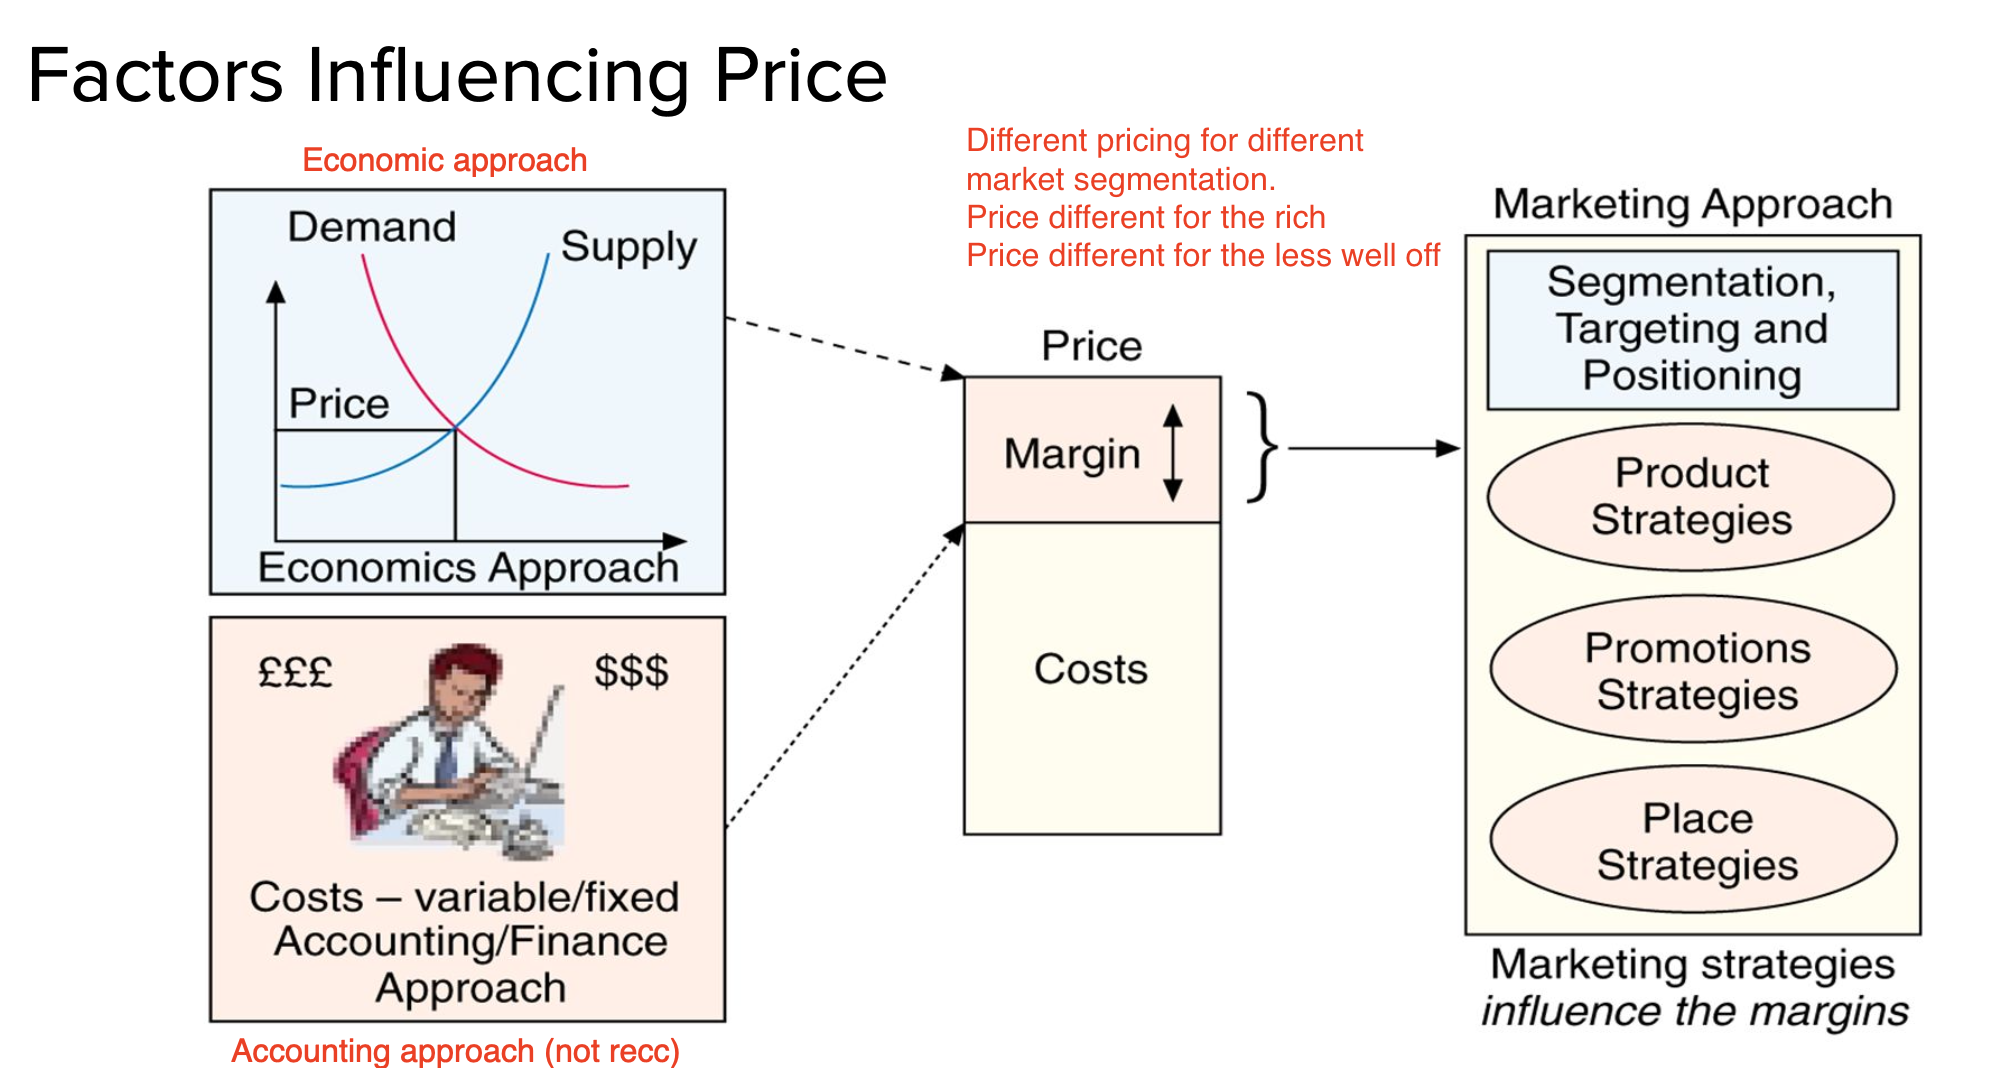
\includegraphics[width=0.97\linewidth]{../images/price_factors.png}
  \end{itemize}
  
  \subsection{Internal Factors Affecting Price}
  \begin{itemize}
    \item \textbf{Marketing Objectives}:
    \begin{itemize}
      \item Survival: Set prices low to cover costs and stay in business
      \item Maximise current profit: Set price to maximise short-term profits, ignore long-term effects
      \item Market share leadership: Set prices low to gain market share
      \item Product quality leadership: Set prices high to reflect high quality
      \item Competitive entry barriers: Set prices to keep out new competitors
      \item Reseller support: Set prices to help resellers make profits
      \item Cost recovery (non-profit \& public firms): Set prices to recover costs
    \end{itemize}
    \item \textbf{Marketing Mix Strategy}:
    \begin{itemize}
      \item Product Design: Higher quality products can support higher prices
      \item Distribution: More intermediaries increase costs and prices
      \item Promotion: Heavy promotion increases costs and prices
      \item Prive vs Non-Price Competition: If competitors use non-price competition, firm has more freedom to set prices. If possible, avoid price wars
      \item Parrellel Importers: Prevent parallel imports by setting similar prices across countries
    \end{itemize}
    \item \textbf{Cost Considerations}:
    \begin{itemize}
      \item Costs set the \textbf{floor} for prices
      \item Demand and competition set the \textbf{ceiling} for prices
      \item Type of costs: Fixed, Variable, Total, Average, Marginal
      \item Marginal cost: Variable cost of producing one more unit of a product
      \item Don't set your price lower than \textbf{marginal cost}.
    \end{itemize}
    \item \textbf{Experience Curves}:
    \begin{itemize}
      \item As production experience increases, unit costs decrease
      \item Combined effects of learning, volume, investment, and specilization lead to cost reductions (e.g . labour efficiency, product design, process engineering)
      \item Exponential decay relationship between unit cost and cumulative production
    \end{itemize}
    \item \textbf{Organisational Considerations}: Who sets the price?
  \end{itemize}

  \subsection{External Factors Affecting Price}
  \begin{itemize}
    \item \textbf{Market and Demand}:
    \begin{itemize}
      \item Form of Competition: Pure, Monopolistic, Oligopolistic, Monopoly
      \item \textbf{Price Elaticity of Demand}: Measure of sensitivity of demand to changes in price
      \item Elastic Demand: Small change in price leads to large change in demand (e.g. luxury goods)
      \item Inelastic Demand: Large change in price leads to small change in demand (e.g. necessities)
      \item Cross-Elasticity of Demand: Measure of sensitivity of demand for product A to changes in price of product B (e.g Apple's ecosystem)
    \end{itemize}
    \item \textbf{Consumer perception}
      \begin{itemize}
        \item Price-Quality Relationship: Consumers associate higher prices with higher quality
        \item Price used in absence of other cues: When consumers have little knowledge about a product, they rely more on price as an indicator of quality
      \end{itemize}
    \item \textbf{Competitor's Strategies and Prices}:
    \begin{itemize}
      \item Reference point: Consumers use competitor's prices as reference points
      \item Responsiveness: Competitors may quickly match price changes
      \item Product homogeneity: If products are similar, price competition is more intense/sensitive. Try to create heterogeneity to not be easily comparable
    \end{itemize}
    \item \textbf{Other External Factors}:
    \begin{itemize}
      \item Economy: Inflation, recession, interest rates affect consumer purchasing power
      \item Distribution Channels: Intermediaries may have their own pricing strategies
      \item Government: Regulations, taxes, tariffs can impact pricing decisions
    \end{itemize}
  \end{itemize}

  \subsection{Methods and Strategies}
  \begin{itemize}
    \item \textbf{Price Skimming}:
    \item \begin{itemize}
      \item Set high initial price to "skim" maximum revenues from segments willing to pay the high price, then lower price over time
      \item Company makes fewer but more profitable sales
      \item Effective when:
      \begin{itemize}
        \item Segmentation on price elasticity: Some customers willing to pay high price
        \item Image supportive: High price supports product's quality and image
        \item Safety/Hedge: High initial price helps recover R\&D costs quickly
        \item Cost of smaller volume cannot be so high that it cancels the advantage of charging more
        \item No immediate competition
      \end{itemize}
    \end{itemize}
    \item \textbf{Penetration Pricing}:
      \begin{itemize}
        \item Set low initial price to penetrate market quickly and deeply, attracting a large number of buyers and market share
        \item Effective when: Consumers are price sensitive, experience curve effects operative, potential competition is high
      \end{itemize}
    
    \item \textbf{Cost-Oriented Pricing}:
      \begin{itemize}
        \item Predetermined markup on cost to ensure a profit
        \item Neglects demand and competitor prices
        \item Markup = (Price - Cost) / Cost
        \item Markup based on sales = (Price - Cost) / Price
        \item \textbf{Target Return/Target Profit Pricing}: Set price to achieve a target return on investment (ROI) or target profit. Requires good demand estimates, $X$.
        \item \( P = DVC + \frac{FC}{X} + \frac{rK}{X} \). Where:
        \item P = Price
        \item DVC = Direct Variable Cost per unit
        \item FC = Fixed Costs
        \item X = Standard Volume
        \item r = Desired rate of return
        \item K = Capital used
      \end{itemize}

    \item \textbf{Demand-Oriented Pricing}
    \item \textbf{Perceived Value Pricing}
    \item \textbf{Odd/Psychological Pricing}: Setting prices that have a psychological impact (e.g. \$9.99 instead of \$10)
    \item \textbf{Lost-Leader Pricing}: Setting prices below cost to attract customers to buy other products
    \item \textbf{Optional-Product Pricing}: Setting prices for optional or accessory products along with a main product
    \item \textbf{Captive-Product Pricing}: Setting prices for products that must be used along with a main product (e.g. razor and blades)
    \item \textbf{Bundled Pricing}: Setting a price for a set of products that is lower than the total of individual prices
    \item \textbf{Price Discrimination}: Time (Peak vs Off-Peak), Location (Theatre vs Home), Customer Segment (Student vs Regular)
  \end{itemize}

\end{multicols*}

\end{document}
